%Capítulo 3

\section{Diseño de la propuesta}

    La parte del backend del sistema de investigadores se compondrá de la siguiente figura \ref{fig:architecture}:
    
    \begin{figure}[H]
        \centering
        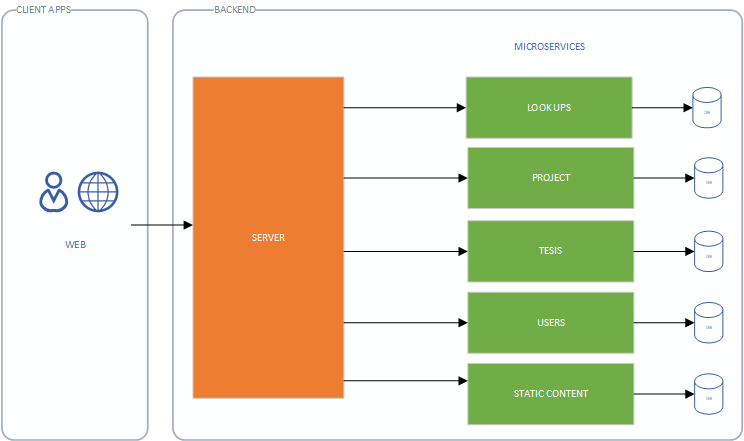
\includegraphics[width=\textwidth]{Propuesta_Plantilla_Tesis_LaTeX_UAG/imagenes/ARCHITECTURE.png}
        \caption{Arquitectura basada en micro servicios.}
        \label{fig:architecture}
    \end{figure}
    
    Con base en la figura \ref{fig:architecture} podemos apreciar que el backend va a responder a una petición hecha a través del usuario usando una interfaz gráfica, acto seguido el servidor identificará la petición para direccionarla al micro servicio correspondiente y esta hará una consulta a la base de datos para poder satisfacer la petición.
    
    Hay distintos tipos de petición que un usuario puede realizar al backend, dentro de estos se encuentran los siguientes verbos o métodos HTTP:
    
    \begin{itemize}
        \item GET: Se utiliza como lectura de datos.
        \item POST: Para poder crear nuevas entradas en la base de datos.
        \item PUT: Para la modificación de datos.
        \item DELETE: Para el borrar datos.
    \end{itemize}
    
    Los distintos tipos de usuarios que existirán son dos: Alumno e Investigador, los cuales tendrán diferentes tipos de participaciones dependiendo del trabajo al que se asignen; mostrados en la figura \ref{fig:users_table}.
    
    \begin{figure}[H]
        \centering
        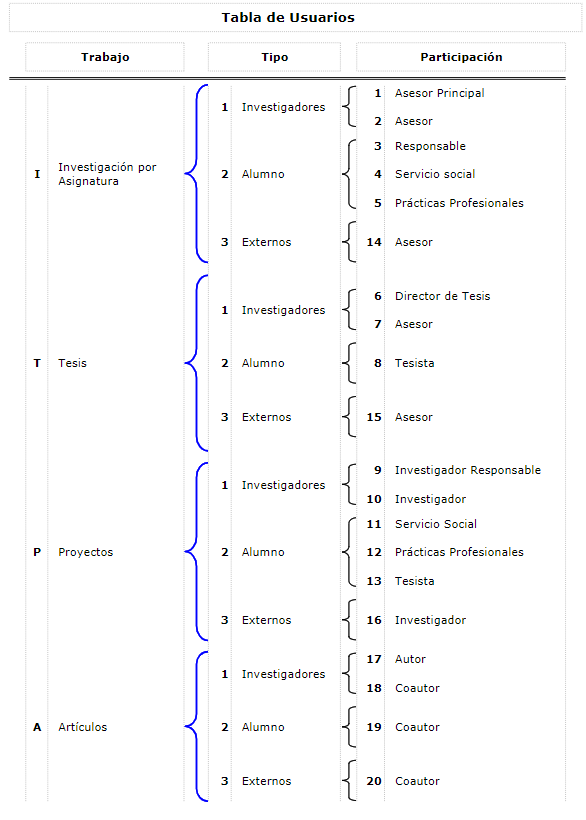
\includegraphics[width=\textwidth]{Propuesta_Plantilla_Tesis_LaTeX_UAG/imagenes/tabla_usuarios.png}
        \caption{Tabla de usuarios ordenada por trabajo y tipo de participación.}
        \label{fig:users_table}
    \end{figure}
    
    Dentro de los posibles flujos para un usuario que quiere consultar todas las tesis registradas para un alumno se puede apreciar en la figura \ref{fig:getAllTesisFromStudents} y sus pasos son los siguientes:
    
    \begin{enumerate}
        \item Realizar la petición al servidor.
        \item El servidor direccionará la petición al micro servicio o API correspondiente por medio de la URI.
        \item El micro servicio resolverá la petición del usuario y dará una respuesta con base en los datos proporcionados en la petición.
        \item El servidor obtendrá la respuesta y la regresará al usuario a través del frontend.
    \end{enumerate}
    
    \begin{figure}[H]
        \centering
        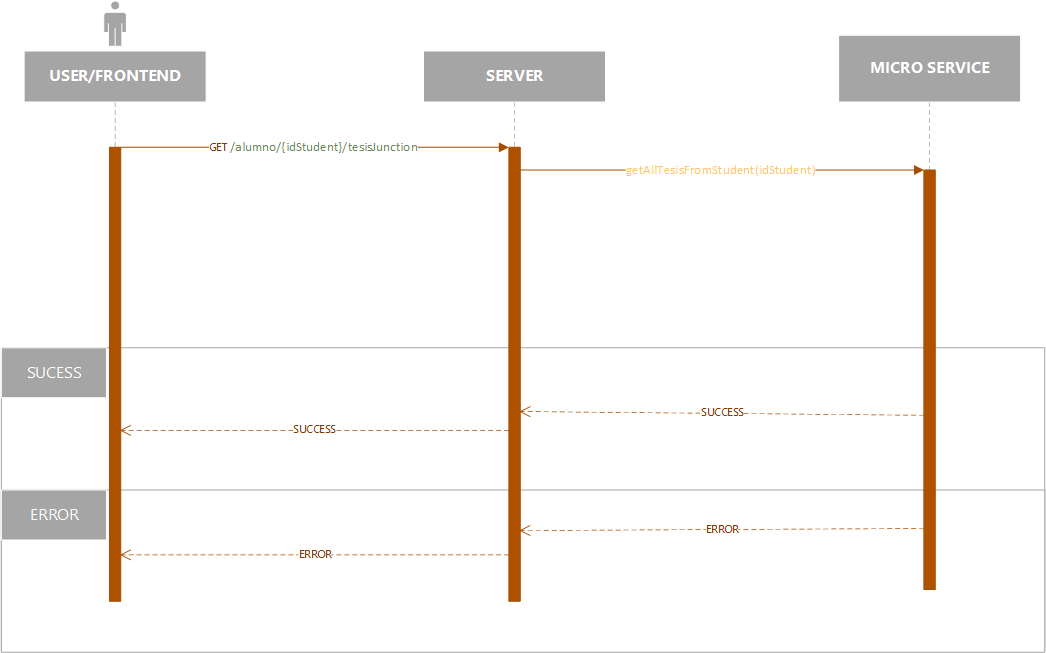
\includegraphics[width=\textwidth]{Propuesta_Plantilla_Tesis_LaTeX_UAG/imagenes/getAllTesisFromStudents_sequence_diagram.png}
        \caption{Diagrama UML para la secuencia de obtener las tesis de un alumno.}
        \label{fig:getAllTesisFromStudents}
    \end{figure}
    
    Se debe plantear un diagrama general de la propuesta del
    proyecto a realizar.
    • El objetivo es explicar en uno o varios diagramas la
    propuesta del proyecto a desarrollar, indicando el flujo de
    información, los módulos principales, la teoría relacionada,
    y los resultados esperados.
    • Debe incluir una relación lógica de los elementos que se
    consideran necesarios para dar una visión completa de la
    propuesta.
    • Debe estar orientado a los objetivos propuestos y debe
    responder a las exigencias teóricas del proyecto.

\section{Metodología}

    Se debe describir tanto la metodología como los pasos a
    seguir para el desarrollo del proyecto.
    • Se presentan los métodos o técnicas existentes a emplear
    para alcanzar los objetivos propuestos
    • Se describe cómo se hará el diseño y el desarrollo de la
    propuesta.
    • Se plantea cuál es el ambiente para realizar los
    experimentos de la propuesta.
    • Se indica cómo se evaluará el alcance de los objetivos.


\section{Cronograma}
Es la planificación y logística que se destinará a cada una
de las etapas de la investigación.
• Es el plan de actividades que muestra un orden lógico y
secuencial del proceso del proyecto.
• Deben señalarse las actividades que serán necesarias
desarrollar para cada etapa de la investigación.
• Comprende desde la presentación del protocolo hasta la
entrega del borrador de tesis.
• Se deben establecer las actividades en función del tiempo
disponible, recursos, materias que se están cursando y
políticas institucionales.

Se debe realizar un calendario tentativo de las actividades
indicadas en la metodología, indicando claramente las
tareas a desarrollar, por etapas, las cuales deberán tener un
estado actualizado (en curso, concluida).
• Se debe tener en cuenta el tiempo que se dedicará a cada
actividad. Aunque parece un detalle menor, este indicará la
factibilidad de realizar el proyecto en el tiempo determinado.
• Se deben indicar las actividades secuenciales o
dependientes y simultáneas.

Debe responder, entre otras, a las siguientes preguntas:
- ¿Cuándo se hará la recopilación de datos?
- ¿Cuándo se hará el diseño y el desarrollo (hardware o
software)
- ¿Cuándo se escribirá la tesis?
- ¿Cuándo se defenderá la tesis?

\section{Entregables}
Indicar los productos derivados del proyecto.
• Se consideran entregables los siguientes:
1. Documento Final (Tesis, Proyecto Intervención)
2. Presentación de avances en seminarios y coloquios.
3. Publicación de avances y resultados en congresos.
4. Artículos de investigación en revistas especializadas.
5. Artículos en revistas de divulgación.
6. Libros y capítulos de libros de resultados obtenidos.
7. Desarrollos y transferencias tecnológicas derivados.
8. Manuales de procedimientos.
9. Patentes, modelos de utilidad.
10. Código